\chapter{Testing}

	After the back end code and the initial front end of the Metric Builder, 
	API and API Documentation features were complete, our team decided to receive 
	user feedback to see where we could improve our design. We created a two part 
	user study to first test the usability, intuitiveness, and simplicity of the 
	Metric Builder's user interface and finally to test the clarity and completeness 
	of API Documentation and to make sure there are no errors in the code samples 
	or the natural language text within the documentation. 

	\section{User Testing Procedure}

		All of the users were students from WPI and were asked to complete the user tasks on a 
		laptop provided by our team. Even though the users in our study are not the typical 
		expected users of the MATTERS site, we believe that their input is valuable. 
		If the features of the site are easy to use for users inexperienced with the MATTERS site, 
		then we should expect the features to be easy for the authorized users in the future as they 
		are more experienced with the MATTERS site or with developing APIs. After completing the tasks 
		for each part of the user study, the users filled out a survey asking them to rate the 
		easiness of different aspects of the tasks on a scale of one to five. While the users were 
		completing their tasks, our team was also there observing their actions in order to get better 
		insight on their clicking behavior and thought process while navigating the site. 
		We also recorded the operating system and browser the users were doing the study on to 
		note any important differences this may bring about.

		\subsection{User Tasks} 
		
			The user tasks given to the users in the following order and were printed on a 
			sheet of paper so that the users could reference the task details at any time:
			
			User Study Tasks: Part 1, Metric Builder feature
			\textit{
				\begin{enumerate}[itemsep=-1.5mm]
					\item
						Navigate to the “Metric Builder” feature
					\item
						Please create your own metric formula, which includes \emph{Unemployment Rate}, 
						\emph{Corporate Income Tax Rate} and \emph{Median Household Income}, 
						with weights \emph{10}, \emph{5}, and \emph{22} respectively.
					\item
						Name your new metric \emph{"My Metric"} and save it.
					\item
						Please find and select your created metric on the “Data Explorer” page.
					\item
						Edit your metric formula so that Unemployment Rate is no longer a part 
						of the metric and Median Household Income has a weight of 15.
					\item
						Save your changes to “My Metric”.
					\item
						Please delete “My Metric”
					\item
						You will now receive a short survey about your 
						experience using the Metric Builder.	
				\end{enumerate}
			}
			
			User Study Tasks: Part 2, API feature and Documentation
			
			\textit{
				\begin{enumerate}[itemsep=-1.5mm]
					\item
						Navigate to the API Documentation page
					\item
						Your API Key is \emph{"secret"}
					\item
						Please get the data for the metric \emph{Unemployment Rate} for \emph{Massachusetts} 
						and \emph{Florida} for the year \emph{2012} using the API tool and the documentation as a guide
					\item
						You will now receive a short survey to complete about your 
						experience using the API and API Documentation.
				\end{enumerate}
			}
			
			The survey that the users completed at the end of each part of 
			the user study can be found in Appendix 2.
		
	\section{Results}

		Thirteen users completed the user study and filled out the subsequent surveys. 
		Most users performed the tasks on Google Chrome or Safari and all users performed 
		the tasks on either a Mac Operating System or Windows Operating System. 
		All of the data collected from the user studies can be found in Appendix 2. 
		Table \ref{metrictest} shows the average of the users' ratings on a scale of 
		one to five for each question on the survey regarding the Metric Builder feature.
		
			\begin{table}[t]
				\centering
				\begin{tabularx}{\textwidth}{@{} Y c @{}} % use 'Y' for first column 
					\toprule
					Survey Question																& Average User Rating	\\
					\midrule
					
					How easy was it to find the Metric Builder?									& 4.385					\\
					How easy was it to select the metrics "Unemployment Rate", 
					"Corporate Income Tax Rate", and "Median Household Income" 
					in the Metric Builder?														& 4.308 				\\
					How easy was it to weigh the metrics accordingly?							& 4.615					\\
					How easy was it to name and save your metric? 								& 5.000					\\
					How easy was it to find “My Metric” on the Data Explorer page? 				& 4.231					\\
					How easy was it to edit “My Metric” to make the appropriate changes?		& 3.846					\\
					How easy was it to remove “My Metric”?										& 5						\\
					
					\bottomrule
				\end{tabularx}
				\caption{Average ratings for the user study on the Metric Builder}
				\label{metrictest}
			\end{table}		
		
		Table \ref{apitest} shows the average of the users' ratings on a scale of one to five for each question on the survey regarding the API Documentation.
			
			\begin{table}[t]
				\centering
				\begin{tabularx}{\textwidth}{@{} Y c @{}} % use 'Y' for first column 
					\toprule
					Survey Question																& Average User Rating	\\
					\midrule
					
					How easy was it to find the API Documentation?								& 3.250					\\
					How useful is the API Documentation?										& 4.167					\\
					
					\bottomrule
				\end{tabularx}
				\caption{Average ratings for the user study on the API Documentation}
				\label{apitest}
			\end{table}	
		
		Our team considered an average rating of above four to be a good score, 
		meaning that the specific task was easy to perform with our user interface.
		The only tasks that did not score above our desired rating was for 
		“How easy was it to edit 'My Metric' to make the appropriate changes?” 
		and “How easy was it to find the API Documentation?”. User feedback on the 
		open ended survey responses, as well as observations made by our team during 
		the user studies were able to confirm that these two tasks were the most 
		difficult or confusing and provided insight as to how to improve it.
		
		For the Metric Builder, users noted that they wanted an option to 
		allow them to edit their metric from the Data Explorer page. 
		Our observations confirmed that while on the Data Explorer page, 
		users were actively searching for an edit button while they were 
		viewing their custom made metric. Many times the users would find the 
		"Create new metric” link quickly, which if clicked would bring the 
		user to the Metric Builder page where they could also edit their metric, 
		but were hesitant to click the link because they were not 
		interested in starting over with a new metric.
		
		For the API Documentation, many users commented on their difficulty finding 
		the link for the API Documentation page. Ultimately, twelve out of the thirteen 
		users did not have much of an issue eventually navigating to the API Documentation 
		link found on the “How to use MATTERS” page as seen in Figure \ref{fig:how}; however, it was more 
		time consuming than it should have been and many users clicked on multiple other 
		links before navigating to the correct page. The users who stated that they did not 
		know what an API was mainly looked for the API Documentation link in the main drop-down 
		menu of the site before navigating to the ”About” page, followed by clicking on the 
		link to “How to use MATTERS” and finally finding the API section which led them to 
		the documentation. Most of the users who were aware of what an API was, ultimately 
		navigated to the API Documentation page the same way; however, many of them scrolled 
		to the bottom of the home page of the site looking for a link similar to the “Developers” 
		links found at the bottom of many webpages.
		
			\begin{figure}[t]
				\centering
				\fbox{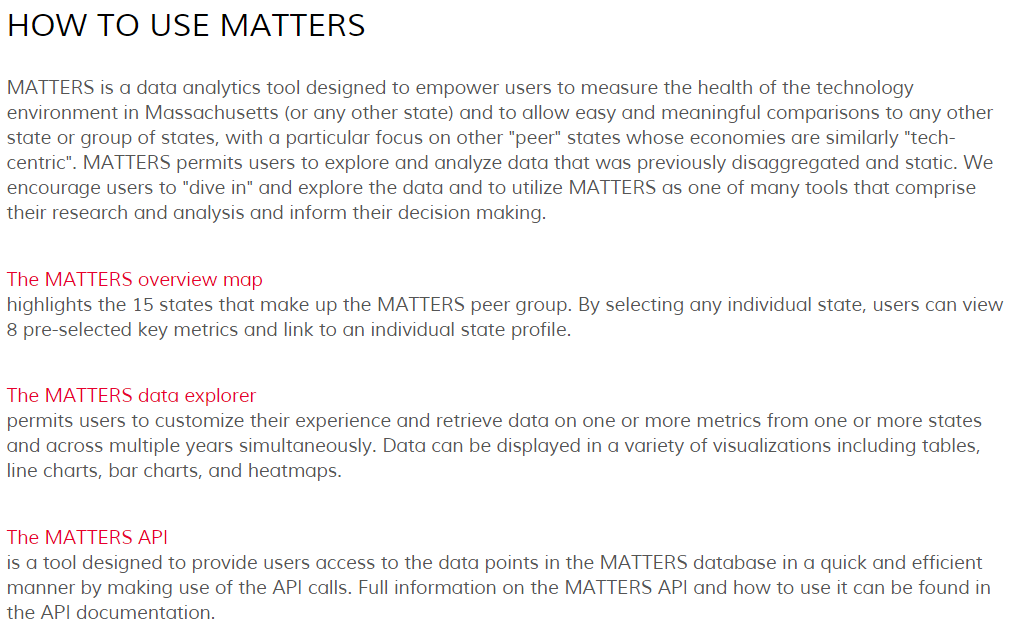
\includegraphics[width=0.75\textwidth]{images/howto.png}}
				\caption{Initial location of the API Documentation link}
				\label{fig:how}
			\end{figure}
		
	\section{Changes made}

		As a result of the user ratings, comments and our observations made while completing 
		the user study tasks, we made a few front end changes to make our features easier 
		to use and easier to find. This included adding a link to the API Documentation in 
		the footer of the site in addition to the link on the "How to use MATTERS" page, as seen 
		in Figure \ref{fig:footer}, and as shown in Figure \ref{fig:edit}, changing the “Create new metric” link on the 
		Data Explorer page to mention that the link would also allow users to edit their metric. 
		
			\begin{figure}[t]
				\centering
					\fbox{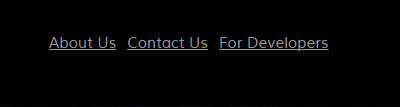
\includegraphics[width=0.75\textwidth]{images/footer.png}}
					\caption{Footer}
					\label{fig:footer}
			\end{figure}
			
			\begin{figure}[t]
				\centering
					\fbox{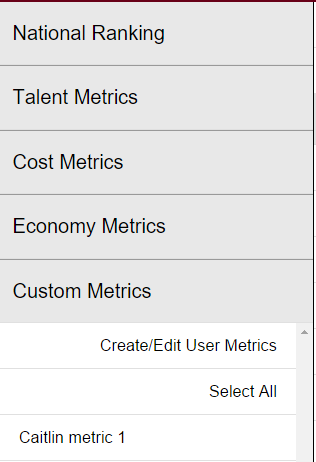
\includegraphics[width=0.5\textwidth]{images/edit.png}}
					\caption{Data Explorer sidebar with edit link}
					\label{fig:edit}
			\end{figure}
			
		These changes led to the final design of the front end of the Metric Builder 
		and API Documentation which can be seen in the figures below. Figures \ref{fig:mb} and \ref{fig:inuse} show the Metric Builder page when a user first visits 
		the page and after a user has selected and assigned weights to some of the metrics from the Metric Selection column of the sidebar. Once the user has decided to save their metric formula, 
		if they choose to go back and edit any part of it, the "Save" button will be replaced by an "Update" button and options are added to "Cancel" any changes or remove the custom metric completely. 
		These additional options can all be seen in Figure \ref{fig:save}. Finally, there were no changes that needed to made to the API Documentation itself as a result of the user testing. 
		Figure \ref{fig:docs}, shows the API Documentation page as it appears when a user first navigate to the page from either the footer or the "How To Use MATTERS" page.

			\begin{figure}[t]
				\centering
					\fbox{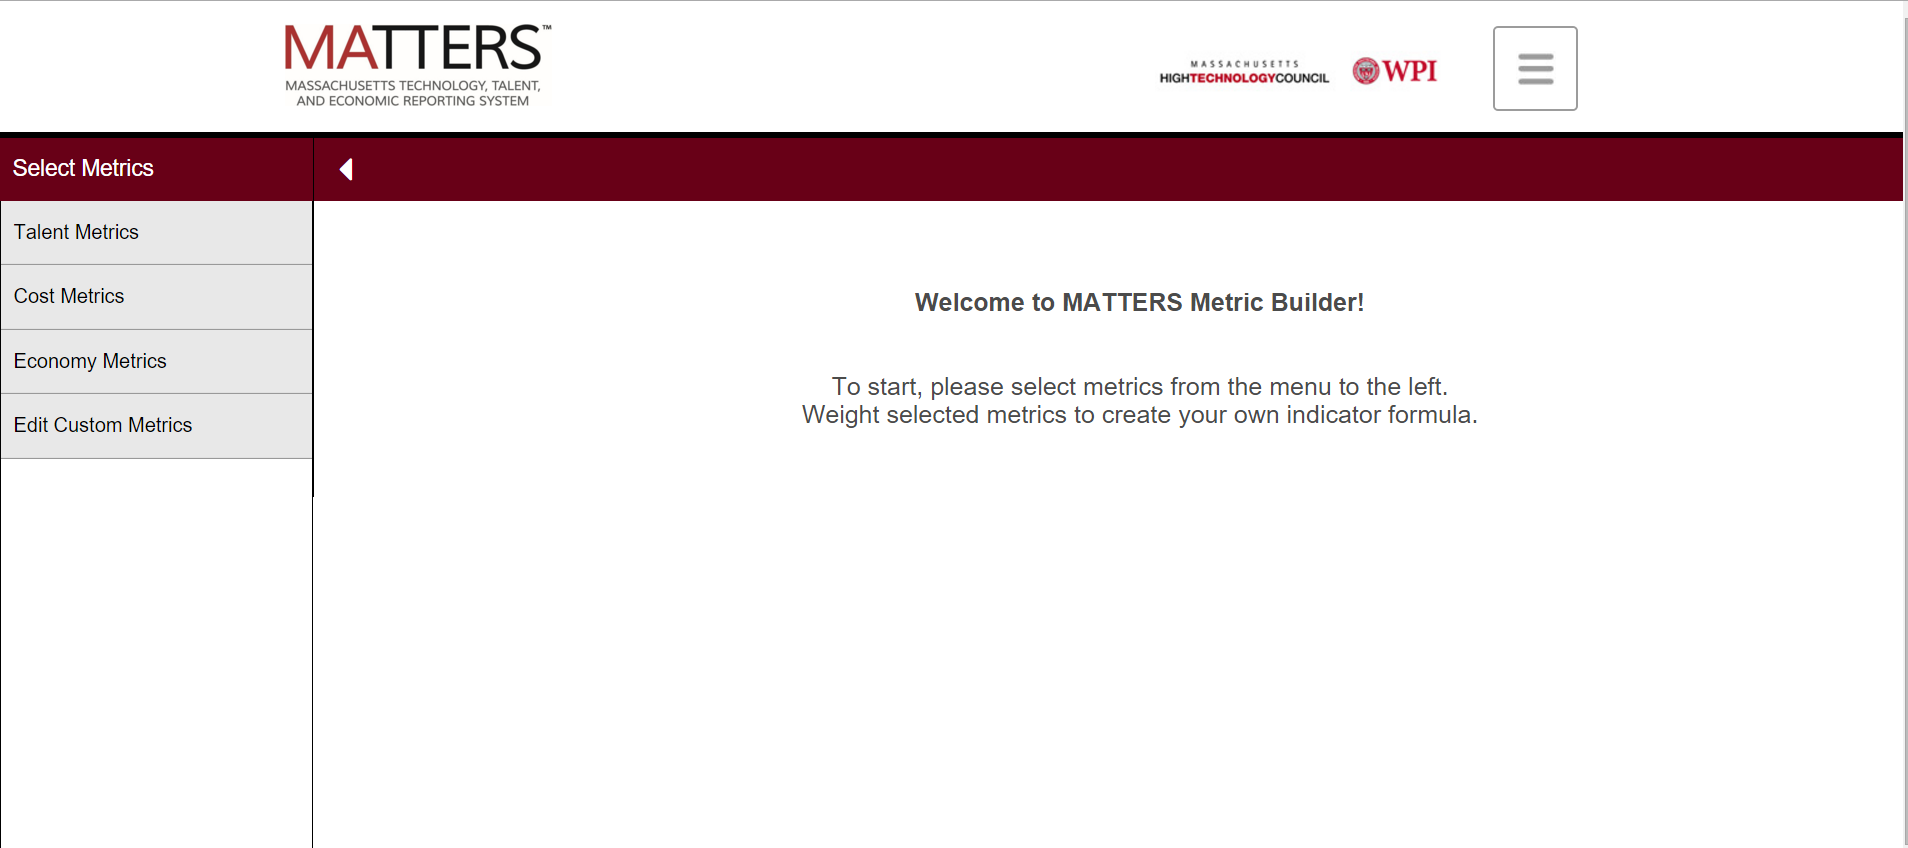
\includegraphics[width=0.75\textwidth]{images/mb.png}}
					\caption{Metric Builder}
					\label{fig:mb}
			\end{figure}
			
			\begin{figure}[t]
				\centering
					\fbox{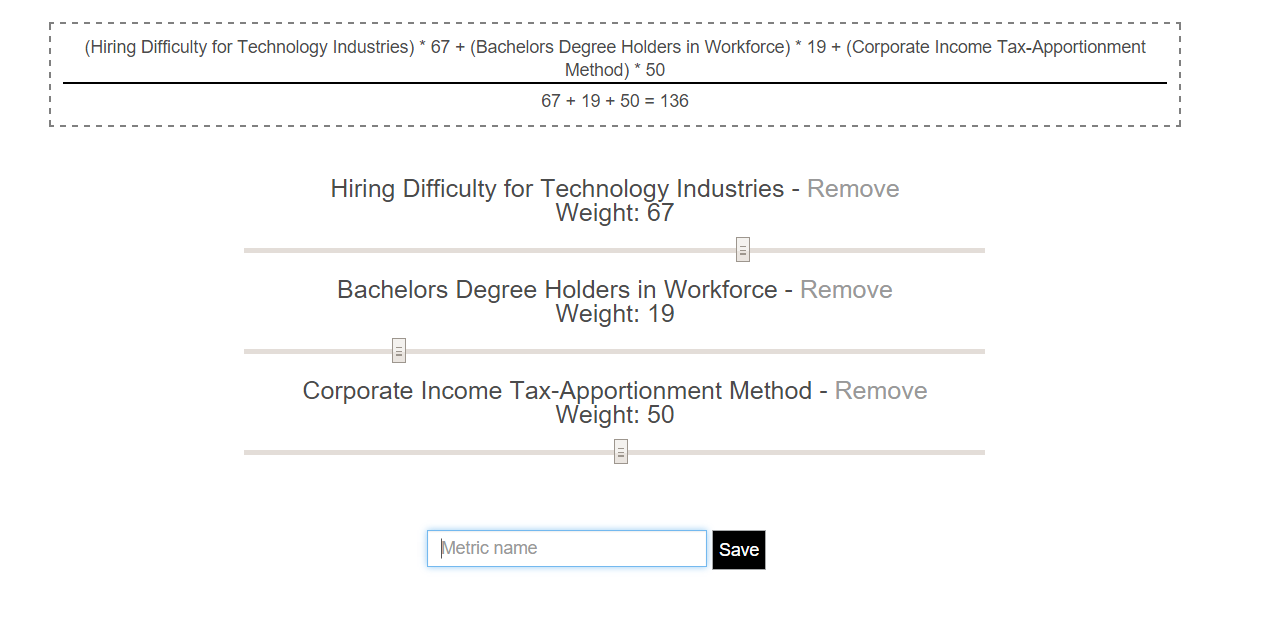
\includegraphics[width=0.75\textwidth]{images/using.png}}
					\caption{Metric Builder's canvas}
					\label{fig:inuse}
			\end{figure}
			
			\begin{figure}[t]
				\centering
					\fbox{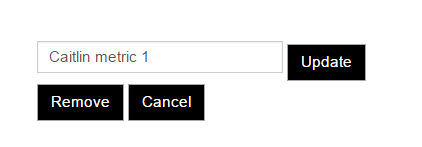
\includegraphics[width=0.75\textwidth]{images/saved.png}}
					\caption{"Save" menu}
					\label{fig:save}
			\end{figure}
			
			\begin{figure}[t]
				\centering
					\fbox{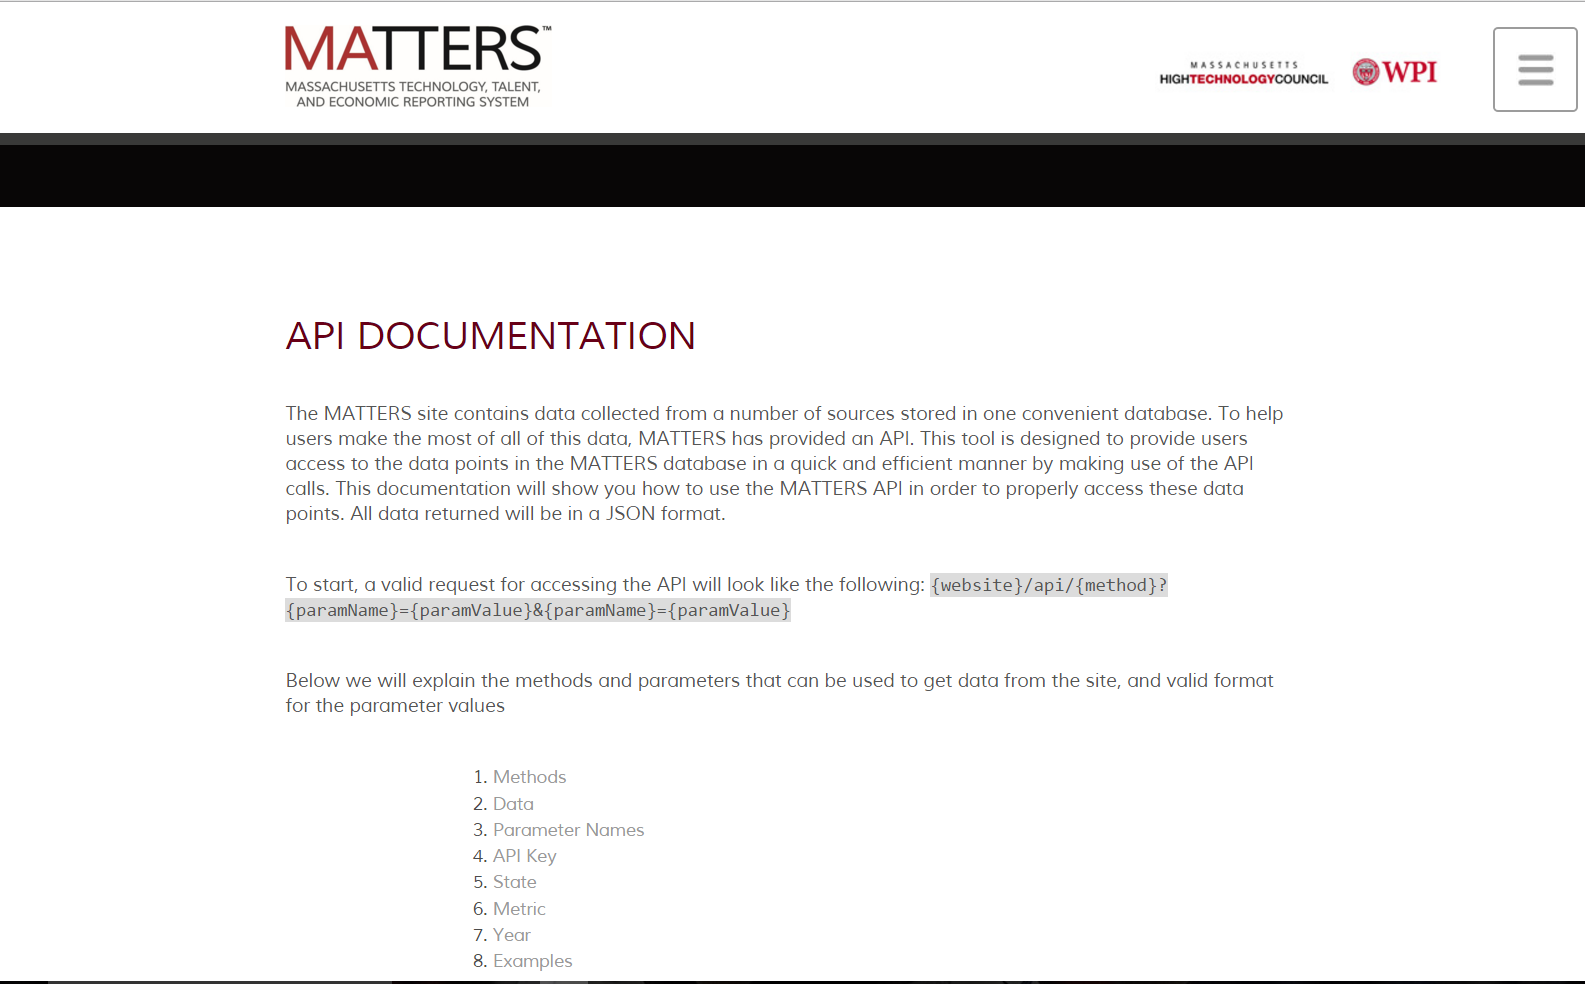
\includegraphics[width=0.75\textwidth]{images/api.png}}
					\caption{API Documentation page}
					\label{fig:docs}
			\end{figure}